\chapter{Modelo Estándar y Supersimetría}
% \addcontentsline{toc}{chapter}{Modelo Estándar y Supersimetría}
\chaptermark{Modelo Estándar y Supersimetría}


El Modelo Estándar (SM, por sus siglas en inglés) es la teoría que describe a las partículas elementales y a sus interacciones. Este modelo fue introducido por Glashow, Salam y Weinberg en la década de los 70 \cite{Glashow:1961tr,Salam:1968rm,Weinberg:1967tq}. Está basado en teorías cuánticas de campo, y sus predicciones, cuantitativas y cualitativas, han sido verificadas experimentalmente con gran precisión.

Una de las extensiones del SM mejor motivada desde el punto de vista teórico es la Supersimetría, ya que resuelve algunas de las limitaciones del mismo. En particular, provee una solución al problema de jerarquía, proporciona candidatos para la materia oscura, permite la unificación de las fuerzas del SM, y hasta propone una conexión entre estas y la gravedad. Es por este motivo, que la Supersimetría, se ha vuelto uno de los objetivos principales en la búsqueda de nueva física en los últimos años.

\section{Modelo Estándar}
 
Según el SM las partículas se clasifican en dos grandes grupos: fermiones y bosones. Los fermiones son los que componen la materia ordinaria y se caracterizan por obedecer la estadística de Fermi-Dirac y tener espín semientero. Estos se clasifican en leptones y quarks, según si experimentan o no la interacción fuerte, siendo los últimos los que pueden interactuar mediante dicha fuerza.  

Existen 6 tipos (o sabores) de leptones que se clasifican en tres generaciones. Cada generación se forma a partir de un leptón masivo y cargado y otro no masivo y neutro. Así se tienen el electrón ($e^{-}$) con su correspondiente neutrino ($\nu_{e}$), y el muón ($\mu^{-}$) y el tau ($\tau^{-}$) con sus neutrinos asociados ($\nu_{\mu}$ y $\nu_{\tau}$ ).


Así mismo, existen 6 tipos de quarks: up ($u$), down ($d$), charm ($c$), strange ($s$), top ($t$) y bottom ($b$). A diferencia de los leptones, lo quarks tienen carga de color, que les permite interactuar mediante la fuerza fuerte. Los quarks solo se manifiestan en estados ligados, denominados hadrones, fenómeno conocido
como confinamiento de quarks. Existen dos tipos de hadrones en la naturaleza: los bariones ($qqq$) y los mesones ($q\bar{q}$).

Los fermiones se pueden encontrar en dos estados de helicidad, izquierda y derecha, salvo los neutrinos que solamente existen en estados de helicidad izquierda. Las dos últimas generaciones de fermiones son inestables, por lo que decaen a las de la primera generación. Es por esto que la materia ordinaria está compuesta por fermiones de la primera generación.

Así como los fermiones están asociados a la materia, los bosones están asociados a los portadores de las interacciones. Los mismos se caracterizan por obedecer la estadística Bose-Einstein y por tener espín entero. Existen cuatro tipos de interacciones fundamentales. La electromagnética, que afecta a las partículas con carga eléctrica, cuyo bosón asociado es el fotón. La débil, que actúa tanto en los quarks como en los leptones, asociada a los bosones $W^{\pm}$ y $Z^{0}$. La interacción fuerte, que actúa en las partículas con carga de color, cuyo portador son los gluones. Finalmente, la cuarta interacción es la gravitatoria. La misma no está descripta por el SM, pero supone que debería actuar sobre todas las partículas del SM y su bosón asociado sería el gravitón.

Todas las partículas anteriormente mencionadas, tienen asociadas una antipartícula con la misma masa y espín, pero con carga y varios de sus números cuánticos opuestos (isospín, charmness, strangeness, topness, número bariónico, etc.). 

El SM se construye formalmente como una teoría de gauge no abeliana, imponiendo invarianza de gauge local sobre campos cuantificados que describen las partículas fundamentales, dando lugar a los campos de gauge que describen las interacciones. Su grupo de simetría es:

\begin{equation}
\mathcal{G}_{SM}=SU(3)_{C}\times SU(2)_{L}\times U(1)_{Y}
\end{equation}

\noindent
donde $Y$ (la hipercarga), $L$ (la helicidad izquierda) y $C$ (la carga de color) representan las cantidades conservadas del grupo de simetría. El subgrupo $SU(2)_{L}\times U(1)_{Y}$ representa el sector electrodébil (QED + interacción débil) y el subgrupo $SU(3)_{C}$ incluye la cromodinámica cuántica (QCD).


En el SM las partículas adquieren su masa mediante el mecanismo de Brout-Englert-Higgs (BEH) \cite{Englert:1964et,Higgs:1964ia,Higgs:1964pj,Guralnik:1964eu,Higgs:1966ev,Kibble:1967sv} , a partir de la ruptura espontanea de la simetría electrodébil:

\begin{equation}
\mathcal{G}_{SM}\rightarrow SU(3)_{C}\times U(1)_{Q}
\end{equation}

\noindent
produciendo los bosones masivos $W^{\pm}$ y $Z^{0}$. Como consecuencia, es necesario incluir en el lagrangiano un nuevo campo escalar, dando lugar a un nuevo bosón masivo de espín 0, llamado bosón de Higgs. El mismo fue descubierto en el año 2012 por las colaboraciones ATLAS y CMS \cite{Aad:2012tfa, Chatrchyan:2012xdj}. La medida más reciente de su masa se determinó con un valor de $125.09 \pm 0.21 (\text{estad.}) \pm 0.11 (\text{sist.}) \gev$ \cite{Aad:2015zhl}. Así como los bosones de gauge adquieren su masa mediante este mecanismo, es posible también generar la masa de los fermiones mediante su interacción con el Higgs, completando de esta forma el espectro de masas del SM. La Tabla \ref{smparticles} expone algunas propiedades de las partículas mencionadas.

\renewcommand{\arraystretch}{1.3}
\begin{table}	
\centering
\caption{Partículas elementales del SM.}
\begin{tabular}{ l | c  c  c | c c }

	\hline

		& \multicolumn{3}{c}{Partículas} & Espín & Carga eléctrica \\

	\hline

	\multirow{3}{*}{Quarks} & $(u,d)_{L}$ & $(c,s)_{L}$ & $(t,b)_{L}$ & $(\frac{1}{2},\frac{1}{2})$ & $(\frac{2}{3},-\frac{1}{3})$ \\

							& $u_{R}$ & $c_{R}$ & $t_{R}$ & $\frac{1}{2}$ & $\frac{2}{3}$ \\

							& $d_{R}$ & $s_{R}$ & $b_{R}$ & $\frac{1}{2}$ & $-\frac{1}{3}$ \\

	\hline

	\multirow{2}{*}{Leptones} 	& $(\nu_{e},e^{-})_{L}$ & $(\nu_{\mu},\mu^{-})_{L}$ & $(\nu_{\tau},\tau^{-})_{L}$ & $(\frac{1}{2},\frac{1}{2})$ & $(0,-1)$ \\

								& $e_{R}^{-}$ & $\mu_{R}^{-}$ & $\tau_{R}^{-}$ & $\frac{1}{2}$ & $-1$ \\

	\hline

	\multirow{3}{*}{Bosones de Gauge} 	& \multicolumn{3}{c |}{$g$} & $1$ & $0$ \\

										& \multicolumn{3}{c |}{$W^{\pm}$, $Z$} & $1$ & $\pm1, 0$ \\

										& \multicolumn{3}{c |}{$\gamma$} & $1$ & $ 0$ \\

	\hline

	Bosones escalares & \multicolumn{3}{c |}{$H$} & 0 & 0 \\

	\hline

\end{tabular}
\label{smparticles}
\end{table}
\renewcommand{\arraystretch}{1}

Como comentario final, el SM tiene 19 parámetros libres: las 9 masas de los fermiones (considerando que los neutrinos tienen masa nula), las 3 constantes de acoplamiento de las interacciones, los 3 ángulos de mezcla de la matriz Cabibbo-Kobayashi-Maskawa (CKM) junto con la fase de la violación CP, el ángulo de vacío de QCD y finalmente la masa del Higgs y su valor de expectación del vacío.


\subsection{Física más allá del Modelo Estándar}

El SM provee una descripción notablemente exitosa de todos los fenómenos accesibles con los experimentos de altas energías disponibles actualmente. Sin embargo, también se sabe que el SM deja cuestiones sin resolver, tanto desde el punto de vista teórico, como experimental.

Desde el punto de vista teórico, el SM no explica los números cuánticos como la carga eléctrica, el isospín, la hipercarga o el color. Tampoco explica por qué los fermiones izquierdos se agrupan en dobletes y los derechos en singletes, ni por qué hay tres cargas de color, o cuántas generaciones hay. Otro síntoma de incompletitud es la gran cantidad de parámetros libres (19) que deben ajustarse a los datos observados, ya que no resultan de principios teóricos más fundamentales.

Desde el punto de vista experimental, también existen algunos resultados que no pueden acomodarse dentro del SM. Distintos experimentos demostraron que si bien los neutrinos tienen una masa muy pequeña, la misma no es nula. En contraposición con el SM que considera a los mismos no masivos. De todas formas, es posible escribir un término de masa para los neutrinos en el lagrangiano \cite{Drewes:2013gca}. El mismo requiere agregar parámetros adicionales a la teoría y además, de la existencia de neutrinos con quiralidad derecha, que aún no fueron observados.

El SM tampoco provee un candidato para la materia oscura. A partir de la observación del movimiento de las galaxias, se sabe que el mismo no se corresponde con la cantidad de materia observada, y es por eso que se propone la existencia de materia indetectable para los instrumentos astronómicos de medición actuales. La materia oscura debería corresponder entonces a partículas masivas, que interactúen solo débilmente y gravitacionalmente.

El triunfo de la teoría electrodébil, parece indicar que todas las interacciones corresponden a distintas manifestaciones de un único campo unificado y que el SM es una teoría efectiva a bajas energías (del orden de los $100\gev$). Incluso ante la ausencia de la gran unificación de las fuerzas electrodébil y fuerte a una escala muy alta de energía, el SM debería ser modificado para incorporar los efectos de la gravedad a la escala de Planck $M_{P} \simeq 10^{19} \gev$. En este contexto, es un misterio por qué la relación $M_{W}/M_{P} \simeq 10^{-17} \gev$ es tan pequeña, lo que se denomina <<problema de jerarquía>>\cite{PhysRevD.14.1667}. Esto lleva a pensar que los fenómenos de nueva física existen 17 órdenes de magnitud por arriba de la energía explorada en el presente. Asociado a este problema está el llamado <<problema de naturalidad>>, donde no se comprende por qué la masa del Higgs es tan pequeña comparada con masa de Planck.


\subsection{Divergencias cuadráticas}

Como se mencionó anteriormente, el SM ha tenido un gran éxito en la descripción de los fenómenos conocidos hasta la escala del TeV. Aun así, es clara la necesidad de construir una nueva teoría que solucione los problemas que el SM conlleva. El principal inconveniente es solucionar el <<problema de jerarquía>>, en el cual el cociente de escalas $M_{W}/M_{P}$ es muy pequeño. Para ello es necesario ver las consecuencias de esta diferencia de escalas.

La parte eléctricamente neutra del campo de Higgs del SM es un escalar complejo $H$ con un potencial clásico $V=m_{H}^{2}|H|^{2}+\lambda|H|^{4}$. El SM necesita un valor de expectación de vacío (VEV) para $H$ no nulo, en el mínimo del potencial. Esto ocurre si $\lambda >0$ y $m_{H}^{2}<0$, resultando en $\left\langle H \right\rangle = \sqrt{-m_{H}^{2}/2\lambda}$. Experimentalmente, de las medidas de las propiedades de las interacciones débiles, se sabe que el valor de $\left\langle H \right\rangle$ es de aproximadamente 174 GeV. El descubrimiento del bosón de Higgs en el 2012 con una masa cercana a 125 GeV implica que, suponiendo que el SM es correcto como una teoría efectiva, $\lambda = 0.126$ y $m_{H}^{2}=-(92.9\: \gev)^{2}$.

Por cada partícula a la que se acopla el campo de Higgs, $m_{H}^{2}$ recibe una gran corrección cuántica de los efectos virtuales. Por ejemplo, si el campo de Higgs se acopla a un fermión $f$ con un término en el lagrangiano igual a $-\lambda H\bar{f}f$, el diagrama de Feynman en la Figura \ref{loops} genera una corrección:

\begin{equation}
\Delta m_{H}^{2}=-\frac{|\lambda_{f}|^{2}}{8\pi^{2}}\Lambda_{UV}^{2}+...
\label{fermion_corr}
\end{equation}

\noindent
donde $m_{f}$ es la masa del fermión y $\Lambda_{UV}$ es el corte usado para regular la integral en el loop. 

\begin{figure}
\centering

	\begin{subfigure}{0.45\textwidth}
	\begin{tikzpicture}
	\begin{feynman}
	\vertex (a) {\(H\)};
	\vertex [right=2cm of a] (b);
	\vertex [above right=of b] (e);
	\vertex [below right=of b] (f);
	\vertex [above right=of f] (c);
	\vertex [right=2cm of c] (d);
	\diagram* {
	(a)-- [scalar] (b),
	(b)-- [fermion, quarter left, edge label=\(f\)] (e),
	(e)-- [quarter left] (c),
	(c)-- [quarter left, fermion] (f),
	(f)-- [quarter left] (b),
	(c)-- [scalar] (d),
	};
	\end{feynman}
	\end{tikzpicture}
	\end{subfigure}
	\hfill
	\begin{subfigure}{0.45\textwidth}
	\begin{tikzpicture}
	\begin{feynman}
	\vertex (a) {\(H\)};
	\vertex [right=3cm of a] (b);
	\vertex [above left=of b] (d);
	\vertex [above right=of b] (f);
	\vertex [above right=of d] (e);
	\vertex [right=3cm of b] (c);
	\diagram* {
	(a)-- [scalar] (b),
	(b)-- [scalar, quarter left] (d),
	(d)-- [quarter left, scalar, edge label=\(S\)] (e),
	(e)-- [quarter left, scalar] (f),
	(f)-- [quarter left, scalar] (b),
	(b)-- [scalar] (c),
	};
	\end{feynman}
	\end{tikzpicture}
	\end{subfigure}

\caption{Correcciones cuánticas a un \textit{loop} al parámetro de masa del Higgs $m_{H}^{2}$ debido a la masa de un fermión de Dirac \textit{f} (izquierda) y debido a la masa de un campo escalar \textit{S} (derecha).}
\label{loops}
\end{figure}

Si $\Lambda_{UV}$ es del orden de $M_{P}$, la corrección a $m_{H}^{2}$ es 30 órdenes de magnitud más grande que el valor requerido $\sim (100\: \gev)^{2}$, produciendo las divergencias cuadráticas. Si bien los fermiones y bosones de gauge no tienen este comportamiento cuadrático en las correcciones cuánticas (sus masas son “naturales”), también se ven afectados indirectamente por este efecto, ya que las masas de los mismos dependen de $\left\langle H \right\rangle$. De esta forma, todas las masas de SM se ven afectadas por la escala de corte $\Lambda_{UV}$.

Una forma de solucionar este problema consiste en considerar la existencia de un escalar complejo $S$ de masa $m_{S}$, que se acopla al campo de Higgs con un término $-\lambda_{S} |H|^{2}|S|^{2}$. El diagrama de Feynman de la Figura \ref{loops} genera una corrección:

\begin{equation}
\Delta m_{H}^{2}=\frac{\lambda_{S}}{16\pi^{2}}\left[\Lambda_{UV}^{2}-2m_{S}^{2}\ln(\Lambda_{UV}^{2}/m_{S})+... \:\right]
\label{boson_corr}
\end{equation}

% \begin{figure}
% \centering
% \begin{tikzpicture}
% \begin{feynman}
% \vertex (a) {\(H\)};
% \vertex [right=3cm of a] (b);
% \vertex [above left=of b] (d);
% \vertex [above right=of b] (f);
% \vertex [above right=of d] (e);
% \vertex [right=3cm of b] (c);
% \diagram* {
% (a)-- [scalar] (b),
% (b)-- [scalar, quarter left] (d),
% (d)-- [quarter left, scalar, edge label=\(S\)] (e),
% (e)-- [quarter left, scalar] (f),
% (f)-- [quarter left, scalar] (b),
% (b)-- [scalar] (c),
% };
% \end{feynman}
% \end{tikzpicture}
% \caption{Correcciones cuánticas a un \textit{loop} al parámetro de masa del Higgs $m_{H}^{2}$ debido a la masa de un campo escalar \textit{S}.}
% \label{loop_f}
% \end{figure}

De esta forma, si existieran fermiones (bosones) no predichos por el SM, relacionados con los bosones (fermiones) del SM mediante una simetría, las contribuciones a las masas de las Ecuaciones \ref{fermion_corr} y \ref{boson_corr} se cancelarían. A esta simetría se la denomina supersimetría (SUSY, por sus siglas en inglés) \cite{Martin:1997ns}.


\section{Extensión Supersimétrica del Modelo Estándar}

Supersimetría es una simetría que relaciona las masas y los acoplamientos de partículas con diferente espín. Una transformación supersimétrica convierte un estado bosónico en uno fermiónico, y viceversa. El operador $Q$ que genera estas transformaciones debe ser un espinor anticonmutativo, que cumpla:

\begin{equation}
\centering
Q \ket{\text{\,bosón\,}} = \ket{\text{\,fermión\,}}
\qquad\qquad\qquad
Q \ket{\text{\,fermión\,}} = \ket{\text{\,bosón\,}}
\end{equation}

Los espinores son intrínsecamente objetos complejos, por lo tanto el conjugado hermítico de $Q$ es también un generador de la simetría. Debido a que $Q$ y $Q^{\dagger}$ son operadores fermiónicos, llevan momento angular de espín $\frac{1}{2}$, por lo tanto es claro que SUSY debe ser una simetría espacio-temporal.

Los estados de partícula de una teoría supersimétrica son representados en el álgebra de SUSY como supermultipletes. Cada supermultiplete contiene ambos estados, fermión y bosón, que son comúnmente llamados supercompañeros uno de otro. Los generadores $Q$ y $Q^{\dagger}$ conmutan con los generadores de las transformaciones de gauge, por lo tanto las partículas en un mismo supermultiplete tienen que estar en la misma representación del grupo de gauge, y tener la misma carga eléctrica, isospín y color. Y como el operador de masa $-P^{2}$ también conmuta con los generadores y con todos los operadores de rotación y traslación, deberán tener los mismos autovalores de $-P^{2}$ , y entonces la misma masa.

Cada supermultiplete tiene que contener igual número de grados de libertad fermiónico que bosónico ($n_{F}=n_{B}$), por lo que existen varias combinaciones posibles. Las dos más importantes para esta teoría son el supermultiplete quiral (o escalar) y el de gauge (o vectorial).

% El supermultiplete escalar tiene un único fermión de Weyl ($n_{F}=2$) y dos escalares reales ($n_{B}=1$). Estos dos escalares se suelen poner como un único campo escalar complejo.

% El supermultplete vectorial contiene un bosón vectorial de spin $1$. Para que la teoría sea renormalizable, tiene que ser un bosón de gauge no masivo, al menos antes de que la simetría de gauge sea espontáneamente rota. En este caso, este bosón contiene dos estados de helicidad ($n_{B}=2$). Por lo tanto su supercompañero es un fermión de Weyl de espín $\frac{1}{2}$, con dos estados de helicidad ($n_{F}=2$). Si en vez de esto, se intenta usar un fermión de espín $\frac{3}{2}$ la teoría no sería renormalizable. Los bosones de gauge deben transformar como la representación adjunta del grupo de gauge, por lo que sus compañeros fermiónicos, llamados <<gauginos>>, también.En el caso de incluir la gravedad, el gravitón de espín 2 (con dos estados de helicidad, n B = 2) tiene un supercompañero de espín llamado <<gravitino>>.

La inclusión de la Supersimetría resuelve varios de los problemas antes mencionados. La simetría cancela las divergencias cuadráticas en la corrección de la masa del Higgs. La corrección de términos de mayor orden requieren que la masa de la partícula supersimétrica más liviana (\textit{Lightest Supersymmetric Particle}, LSP) sea del orden del TeV, siendo ese el orden de energía en el cual el SM deja de ser válido, y es necesaria la implementación de SUSY. También provee un candidato a materia oscura, siendo en la mayoría de los modelos la partícula supersimétrica más liviana, que es estable y no interactuante. Finalmente, SUSY provee un marco de referencia para una teoría de Gran Unificación y para teorías que incorporan a la gravedad. 



\subsection{Modelo Estándar Supersimétrico Mínimo}

Como se mencionó antes, en una extensión supersimétrica del SM, cada una de las partículas elementales conocidas está contenida en un supermultiplete quiral o de gauge, y debe tener un supercompañero con espín que difiera en $\frac{1}{2}$. La extensión que requiere la introducción de la mínima cantidad de parámetros se conoce como <<Modelo Estándar Supersimétrico Mínimo>> (MSSM por sus siglas en inglés).

Veamos ahora como se van construyendo los distintos supermultipletes. Como los supermultipletes escalares son los únicos que pueden contener un fermión cuya parte izquierda y derecha transforman de forma diferente, todos los fermiones del SM están agrupados en este tipo de supermultiplete. En cuanto a su nomenclatura, los nombres de los compañeros de espín 0 de los quarks o leptones son construidos anteponiendo una “s” (de scalar ), y son llamados <<squarks>> y <<sleptones>>. La parte izquierda y derecha de los quarks y leptones son fermiones de Weyl con diferentes propiedades de transformación de gauge del SM, entonces cada uno debe tener un compañero escalar complejo. Por ejemplo, los supercompañeros de la parte izquierda y derecha del campo de Dirac de los electrones son llamadas $\tilde{e}_{L}$ y $\tilde{e}_{R}$ , aunque el subíndice no se refiere a la helicidad de los slectrones (ya que ambos tienen espín 0) sino a la de sus supercompañeros. Lo mismo aplica para las demás leptones y quarks, los neutrino son simplemente denominados $\tilde{\nu}$ ya que son siempre izquierdos.

El bosón escalar de Higgs debe estar en un supermultiplete quiral ya que tiene espín 0. Dada la naturaleza de los campos quirales introducidos en la implementación de SUSY, el campo escalar de Higgs no es suficiente para dar masa a los fermiones de helicidad izquierda y derecha, por lo que se debe agregar un nuevo campo escalar para compensar. En el SM, el campo de Higgs es un doblete, y de los cuatro grados de libertad solo uno permanece como consecuencia de la ruptura de la simetría electrodébil, resultando en un bosón de Higgs. En el MSSM se necesitan dos dobletes de Higgs, $H_{u}=(H^{+}_{u},H^{0}_{u})$ y $H_{d}=(H^{0}_{d},H^{-}_{d})$. El escalar neutro que corresponde al bosón de Higgs del SM es una combinación lineal de $H^{0}_{u}$ y $H^{0}_{d}$. La nomenclatura usual para referirse a los supercompañeros de espín  es agregar “-ino” a la partícula del SM, por lo tanto los compañeros fermiónicos de los escalares de Higgs son denominados <<higgsinos>>, y se denotan $\widetilde{H_{u}}$ y $\widetilde{H_{d}}$.

Los bosones vectoriales del SM tienen que estar en supermultipletes de gauge y sus supercompañeros fermiónicos son llamados <<gauginos>>. Las interacciones de gauge de color de QCD son mediadas por el gluon, cuyo compañero supersimétrico de espín  es el <<gluino>>. Los gauginos supercompañeros de los bosones de gauge electrodébiles, luego de mezclarse con los supercompañeros de los bosones de Higgs, dan lugar a los autoestados de masa denominados <<charginos>> y <<neutralinos>>. En la Tabla \ref{susyparticles} se puede ver el espectro completo del MSSM.


\renewcommand{\arraystretch}{1.3}
\begin{table}	
\centering
\begin{threeparttable}
\caption{Supermultipletes quirales y de \textit{gauge} del MSSM.}
\begin{tabular}{ P{4cm} P{4cm} P{4cm} }

	\hline

	Supermultiplete & Bosón & Fermión \\

	\hline

	gluón, gluino & $g$ & $\widetilde{g}$ \\

	\hline

	W, wino & $W^{\pm}$, $W^{0}$ & $\widetilde{W}^{\pm}$, $\widetilde{W}^{0}$ \\
	B, bino & B & $\widetilde{B}$ \\

	\hline

	\multirow{2}{*}{sleptón, leptón $^{*}$} 	& $(\widetilde{\nu},\widetilde{e}_{L})$ & $(\nu,e_{L})$ \\

										& $\widetilde{e}_{R}$ & $e_{R}$ \\

	\hline

	\multirow{3}{*}{squark, quark $^{*}$}		& $(\widetilde{u}_{L},\widetilde{d}_{L})$ & $(u_{L},d_{L})$ \\

										& $\widetilde{u}_{R}$ & $u_{R}$ \\

										& $\widetilde{d}_{R}$ & $d_{R}$ \\

	\hline

	\multirow{2}{*}{Higgs, higgsinos}	& $(H^{0}_{d},H^{-}_{d})$ & $(\widetilde{H}^{0}_{d},\widetilde{H}^{-}_{d})$ \\

										& $(H^{+}_{u},H^{0}_{u})$ & $(\widetilde{H}^{+}_{u},\widetilde{H}^{0}_{u})$ \\

	\hline
\end{tabular}
\begin{tablenotes}
\item [*] \footnotesize Junto con las otras dos generaciones.
\end{tablenotes}
\label{susyparticles}
\end{threeparttable}
\end{table}
\renewcommand{\arraystretch}{1}


Por construcción, cada partículas y su supercompañero debe tener la misma masa, por lo que deberían existir, por ejemplo, fotinos de masa nula y selectrones con $0.511 \mev$. Como ninguna de las partículas antes mencionada fue observada experimentalmente, se deduce que SUSY es una simetría que está rota en el estado de vacío elegido por la naturaleza.

El hecho de que sea una simetría rota, impide que se cancelen las divergencias cuadráticas en el cuadrado de las masas escalares, y eso fue uno de los motivos por el cual se introdujo SUSY. Para poder garantizar que siga ocurriendo esa cancelación, la ruptura de la simetría debe ser suave, y el lagrangiano efectivo del MSSM tiene que escribirse como:

\begin{equation}
\mathcal{L}=\mathcal{L}_{\text{SUSY}}+\mathcal{L}_{\text{soft}}
\end{equation}

\noindent
donde $\mathcal{L}_{\text{SUSY}}$ contiene todas las interacciones de gauge y de Yukawa, y preserva la invarianza supersimétrica. 
% El conjunto de parámetros que aparecen en el lagrangiano $\mathcal{L}_{SUSY}$ son:

% \begin{itemize}

% 	\item las constantes de acoplamiento de gauge $g_{s}$, $g$ y $g'$ correspondientes a los grupos de gauge $SU(3)_{C}$, $SU(2)_{L}$ y $U(1)_{Y}$, respectivamente

% 	\item los acoplamientos de Yukawa que describen las interacciones entre fermiones y bosones de Higgs

% 	\item el parámetro de masa del campo de Higgs $\mu$.

% \end{itemize}


El lagrangiano que rompe SUSY, $\mathcal{L}_{\text{soft}}$, no está completamente determinado y su forma explícita así como el conjunto de parámetros involucrados dependen del mecanismo particular de ruptura de SUSY. Debido a que este mecanismo es desconocido, se puede suponer un conjunto de términos de ruptura de la forma más general posible, sin indagar en sus orígenes, que se fijan solo pidiendo la invarianza frente $SU(3)_{C}\times SU(2)_{L}\times U(1)_{Y}$, y que sean suaves a fin de mantener la cancelación de las divergencias cuadráticas. Estos términos soft proveen exitosamente las masas de las partículas supersimétricas, a fin de que sean más pesadas que sus correspondientes compañeras del SM, y la ruptura espontánea de la simetría electrodébil requerida a bajas energías necesaria para explicar la generación de las masas de las partículas del SM. Aun así, la diferencia de masa entre supercompañeros no debe ser demasiado grande, ya que se perdería la solución al problema de jerarquía.

% El conjunto de nuevos parámetros que aparece en el superpotencial de ruptura de SUSY incluye \cite{Agashe:2014kda,Haber:1993wf}:

% \begin{itemize}
 
% 	\item Las masas soft del sector de Higgs, $m_{1}$ , $m_{2}$ y $m_{12}$ , donde $m_{12}^{2} \equiv B\mu$, $\mu$ es el parámetro introducido anteriormente y $B$ es el parámetro de ruptura de SUSY.

% 	\item Las masas soft de los squarks y sleptones de cada generación: $m_{\tilde{Q}}$ , $m_{\tilde{U}}$ , $m_{\tilde{D}}$ , $m_{\tilde{L}}$ y $m_{\tilde{E}}$ .

% 	\item Los acoplamientos trilineales de squarks y sleptones $A_{q}$ y $A_{l}$.

% 	\item Las masas soft de los gauginos, $M_{3}$ , $M_{2}$ y $M_{1}$ , asociadas a los grupos de gauge del $SU(3)_{C}$, $SU(2)_{L}$ y $U(1)_{Y}$, respectivamente.

% \end{itemize}

Adicionalmente, para evitar problemas con la conservación del número bariónico $B$ y leptónico $L$, se introduce una nueva simetría denominada paridad-R. Se define como $P_{R}=(-1)^{3(B-L)+2s}$, donde $s$ es el espín de la partícula. Las partículas supersimétricas tienen $P_{R}=-1$, mientras que las partículas del SM tienen $P_{R}=+1$. La conservación de la paridad-R genera que las partículas supersimétricas solo puedan ser producidas en número par en experimentos de colisiones.

El trabajo de la referencia \cite{Dimopoulos:1995ju} muestra que el MSSM posee 124 parámetros independientes. De estos, 18 corresponden a los parámetros del SM, uno corresponde al sector de Higgs (el análogo a la masa del Higgs del SM), y 105 son nuevos parámetros del modelo. 

Existen distintas propuestas para los mecanismos de ruptura de supersimetría. En la búsqueda asociada al presente trabajo, el modelado de la señal de SUSY se da en el contexto del modelo “Generalised Model of Gauge-Mediated Supersymmetry Breaking” (GGMSB). En este modelo, la supersimetría es rota en la escala del TeV en un sector oculto de estados inaccesibles por procesos del SM, y es propagada al sector visible del MSSM vía interacciones de bosones de gauge del grupo $SU(3)_{C} \times SU(2)_{L} \times U(1)_{Y}$ y gauginos.

En estos modelos con mediaciones de gauge, el gravitino es la partícula supersimétrica más ligera (LSP), con masas del orden del keV, estable y no interactuante, produciendo así energía faltante en la reconstrucción del evento en su estado final.

\subsection{El espectro de masas}

Los supercompañeros de las partículas del SM no son necesariamente los estados de masa del MSSM. Incluyendo efectos de ruptura de simetría electrodébil y supersimetría se producen estados de masa como mezcla de gauginos y higgsinos. La única excepción es el gluino que es un octeto de color y no se mezcla con otras partículas.

Las masas y mezclas de las distintas partículas tienen un rol importante en cuanto a su fenomenología y su correspondiente búsqueda experimental, por lo que se describen brevemente a continuación.


\subsubsection{El sector de Higgs} 

El escalar de Higgs en el MSSM consiste en dos dobletes del $SU(2)_{L}$ complejos, $H_{u}$ y $H_{d}$, con ocho grados de libertad reales. Luego de la ruptura de simetría electrodébil, tres de ellos son los bosones de Nambu-Goldstone, que corresponden a los modos longitudinales de los bosones masivos $Z$ y $W^{\pm}$. Los restantes cinco grados de libertad producen el bosón de Higgs físico del modelo. La siguiente nomenclatura es utilizada:
\begin{align*}
  H^{\pm} & : \text{par de bosones de Higgs cargados} \\
  A^{0} & : \text{bosón de Higgs neutral CP-impar} \\
  H^{0},\: h^{0} & : \text{bosones de Higgs neutrales CP-par} 
\end{align*}

Una de las predicciones bastantes sólidas de supersimetría es que debe haber al menos un bosón de Higgs liviano.


\subsubsection{Neutralinos y charginos}

Los higgsinos y los gauginos electrodébiles pueden combinarse debido a los efectos de la ruptura de simetría electrodébil. Los higgsinos neutros ($\widetilde{H}^{0}_{u}$ y $\widetilde{H}^{0}_{d}$) y los gauginos neutros ($\widetilde{B}$ y $\widetilde{W}^{0}$) se combinan para formar cuatro autoestados de masa llamados <<neutralinos>>, denotados $\widetilde{\chi}^{0}_{1}$, $\widetilde{\chi}^{0}_{2}$, $\widetilde{\chi}^{0}_{3}$ y $\widetilde{\chi}^{0}_{4}$, ordenados de forma ascendente por sus masas. El neutralino más liviano, $\widetilde{\chi}^{0}_{1}$, generalmente se considera como la LSP, ya que es una de las partículas del MSSM que puede ser un buen candidato para la materia oscura. 

Los higgsinos cargados ($\widetilde{H}^{+}_{u}$ y $\widetilde{H}^{-}_{d}$) y los winos ($\widetilde{W}^{+}$ y $\widetilde{W}^{-}$) se combinan para formar dos autoestados de masa con carga $\pm1$, denominados <<charginos>> y se denotan $\widetilde{\chi}^{\pm}_{1}$ y $\widetilde{\chi}^{\pm}_{2}$. Ordenados, por convención, de forma ascendente en sus masas.


\subsubsection{Gluino}

El gluino es un fermión de color con ocho componentes, por lo que no puede mezclarse con ninguna otra partícula del MSSM (aunque haya violación de paridad-R). El parámetro de masa ($M_{3}$) está relacionado con los parámetros de masa del bino ($M_{1}$) y el wino ($M_{2}$), con una relación:

\begin{equation}
M_{3}:M_{2}:M_{1} \approx 6:2:1
\end{equation}

\noindent
cerca de la escala del TeV. Por esto mismo, es razonable pensar que el gluino sea considerablemente más pesado que los neutralinos y charginos livianos.


\subsubsection{Squarks y sleptones}

Cualquier par de escalaras con la misma carga eléctrica, paridad-R, color y números cuánticos pueden mezclarse entre ellos. Al agregar el término \textit{soft} en el MSSM, los autoestados de masa de los squarks y sleptones se pueden obtener diagonalizando tres matrices de $6 \times 6$ para squarks up, down y sleptones cargados, y una matriz adicional de $3 \times 3$ para los sneutrinos. La primera y la segunda generación de squarks y slpetones generalmente contiene 7 pares sin mezclar degenerados. En cambio, la tercer generación puede tener masas muy diferentes y combinaciones de pares ($\tilde{t}_{L}$, $\tilde{t}_{R}$), ($\tilde{b}_{L}$, $\tilde{b}_{R}$) y ($\tilde{\tau}_{L}$, $\tilde{\tau}_{R}$). Para un cierto fermión de la tercera generación, la matriz hermítica de masas en la base del autoestado de gauge ($\tilde{f}_{R}$, $\tilde{f}_{R}$) puede ser diagonalizado por una matriz unitaria para producir los autoestados de masa, denotados ($\tilde{f}_{1}$, $\tilde{f}_{2}$).

Debido a la elevada masa del quark top, la combinación es muy fuerte en el sector stop. Esto genera una gran separación entre las masas de los dos autoestados del stop, produciendo un stop mucho más liviano que los demás squarks

Distintos análisis realizados a partir de la toma de datos en el detector ATLAS, obtuvieron límites para las masas de las partículas supersimétricas. La Figura \ref{masses} muestra un resumen de los resultados actuales obtenidos.

\begin{figure}[ht]
\centering
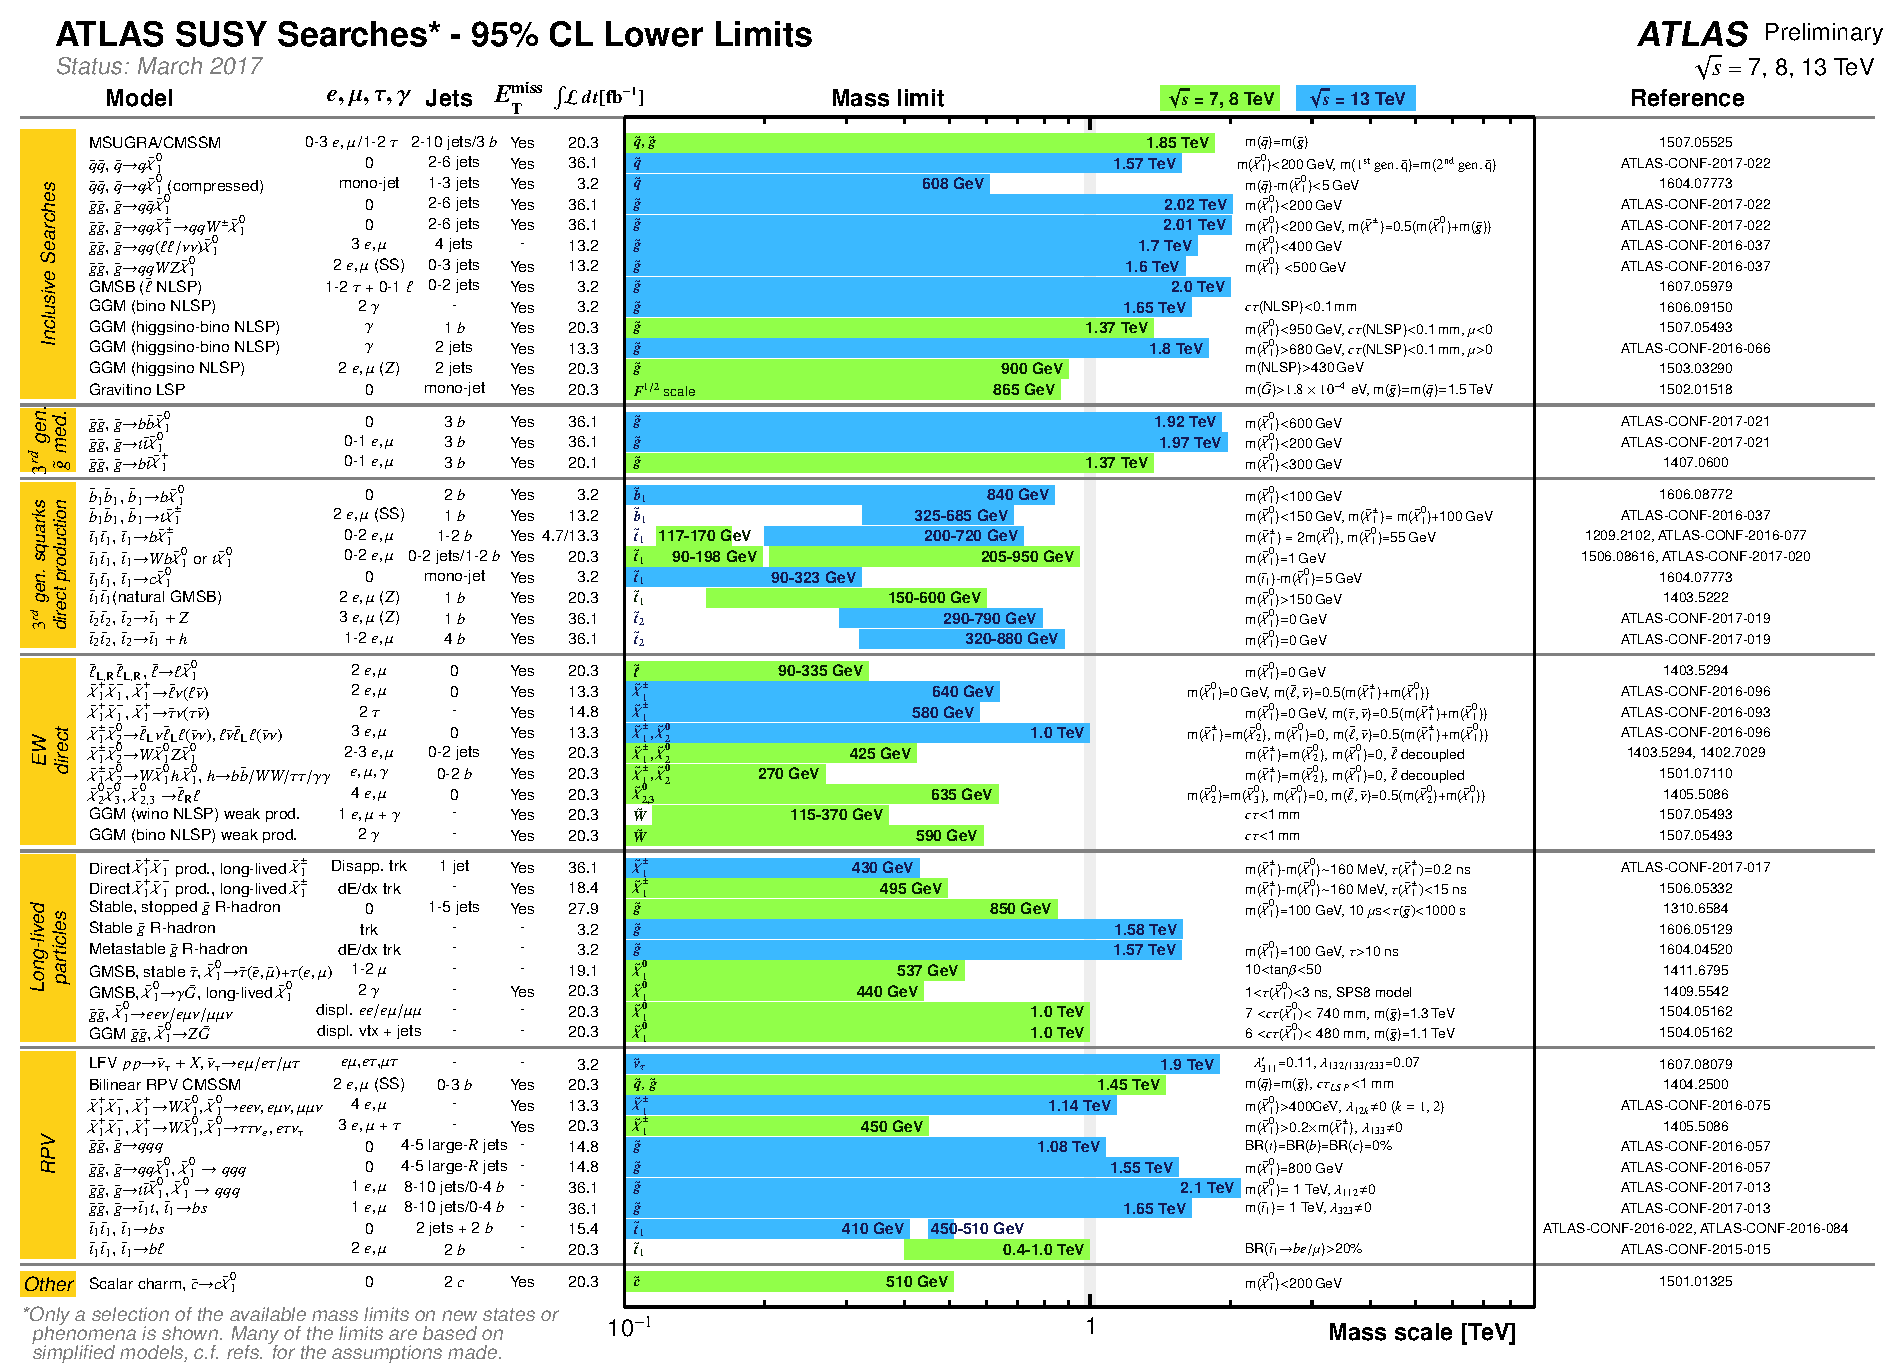
\includegraphics[width=1\textwidth]{images_tmp/masses.pdf}
\caption{Resumen de los límites de exclusión en la masa de las partículas supersimétricas por distintos análisis realizados en ATLAS \cite{masses_web}.}
\label{masses}
\end{figure}



\section{Colisión \textit{pp}}

El LHC es un colisionador de protones, por lo tanto para comprender los procesos que ocurren en el mismo, es necesario entender la estructura del protón. Su composición se puede describir mediante la cromodinámica cuántica (QCD) \cite{ellis1996}, que explica las interacciones entre partículas que poseen carga de color: quarks y gluones. Los mediadores de la interacción, los gluones, pueden interactuar consigno mismo, lo que produce que la fuerza dependa de la distancia entre las cargas. De esta forma, la constante de acoplamiento de la fuerza, aumenta a grandes distancias (o bajas energías) y disminuye para distancias menores (altas energías). Es por este motivo que los cálculos perturbativos solo se pueden efectuar a altas energías. Otra característica de la interacción es el confinamiento, es decir, que las partículas con color no puedan existir libremente. Solo estados de color neutro de múltiples partículas de color pueden ser observados en la naturaleza viajando distancias macroscópicas.

El protón es un barión, compuesto por dos quarks \textit{u} y un quark \textit{d}, cada uno con una carga de color tal que deje al protón en un estado neutro. Estos tres quarks son llamados quarks de valencia del protón, y están rodeados por un mar de gluones y pares de quark-antiquark que surgen de fluctuaciones cuánticas. A altas energías la colisión entre protones se puede considerar como una colisión entre dos de sus constituyentes, aplicando el <<modelo de partones>>. Este modelo fue introducido por Feynman \cite{PhysRevLett.23.1415} y Bjorken \cite{PhysRev.185.1975} a fines de los años 60, para interpretar los resultados de los experimentos de dispersión inelástica profunda (DIS) electrón-nucleón en SLAC. Los quarks de valencia y los quarks y antiquarks del mar junto con los gluones son llamados <<partones>> del protón. Cada partón lleva solo una fracción del momento y la energía del protón. Para la medición de una sección eficaz de dispersión fuerte que involucre quarks y gluones en el estado inicial, es necesario conocer el momento de las partículas incidentes. Como los partones solo llevan una fracción del momento del protón, y están en interacción permanente entre ellos, el momento es desconocido, por lo que la escala de energía de las colisiones varía. Además, como se mencionó, los quarks (\textit{q}) y gluones (\textit{g}) salientes no pueden observarse directamente debido al confinamiento, pero son observados en el detector como jets. Entonces no es posible medir una sección eficaz partónica como $\sigma(qg \rightarrow qg)$, pero se puede hacer una medida inclusiva, como la sección eficaz hadrónica $\sigma(pp \rightarrow jj)$ con dos jets en el estado final. En teoría de perturbaciones, para pasar desde la sección eficaz partónica a la sección eficaz hadrónica es necesario conocer la probabilidad de que un partón de tipo \textit{n} sea encontrado con una fracción de momento \textit{x}, es decir, las funciones de distribución partónica (PDF). Estas funciones son determinadas a partir de datos obtenidos de los propios experimentos de altas energías, ya que no pueden determinarse a partir de la teoría. 

Esta conexión entre los hadrones observables y el nivel partónico es posible gracias al concepto de <<factorización>>, que permite una separación sistemática entre las interacciones de corta distancia (de los partones) y las interacciones de larga distancia (responsables del confinamiento de color y la formación de hadrones). El teorema de factorización \cite{ELLIS1978281} establece que la sección eficaz de producción de cualquier proceso de QCD del tipo $A + B \rightarrow X$, siendo $a_{i}$ ($b_{j}$) los constituyentes del hadrón inicial $A$ ($B$), puede ser expresada como: 

\begin{equation}
\sigma_{AB\rightarrow X}=\sum_{ij}\int dx_{a_{i}}dx_{b_{j}}f_{A/a_{i}}(x_{a_{i}},\mu_{F}^{2})f_{B/b_{j}}(x_{b_{j}},\mu_{F}^{2})\sigma_{a_{i}b_{j}}(\mu_{F}^{2},\mu_{R}^{2})
\end{equation}

\noindent
donde $x_{i}$ ($x_{j}$) es la fracción del momento del hadrón $A$($B$) que lleva el partón $a_{i}$ ($b_{j}$) y $\sigma_{a_{i}b_{j}\rightarrow X}$ es la sección eficaz de la interacción a nivel partónico, calculada a un dado orden de perturbaciones y una escala de renormalización $\mu_R$. La escala de renormalización es introducida para absorber las divergencias ultravioletas que aparecen en los cálculos perturbativos más allá del primer orden. Las funciones $f_{A/a_{i}}(x_{a_{i}},\mu_{F}^{2})$ son las PDF, que representan la probabilidad de encontrar un partón de tipo \textit{n} en el hadrón \textit{h} con una fracción de momento $x_{n}$, dada una escala de factorización $\mu_{F}$. Esta escala es un parámetro arbitrario introducido para tratar singularidades que aparecen en el régimen no perturbativo. Estas divergencias son absorbidas, en forma similar a la renormalización, dentro de las funciones de distribución partónicas a la escala $\mu_{F}$. 


A modo de ejemplo, en la Figura \ref{cross_section}, se muestra el buen acuerdo entre la sección eficaz de algunos procesos del SM medidas por ATLAS y las predicciones teóricas. Las observaciones experimentales realizadas en LHC resultan compatibles con el SM a un nivel de muy alta precisión.


\begin{figure}[ht]
\centering
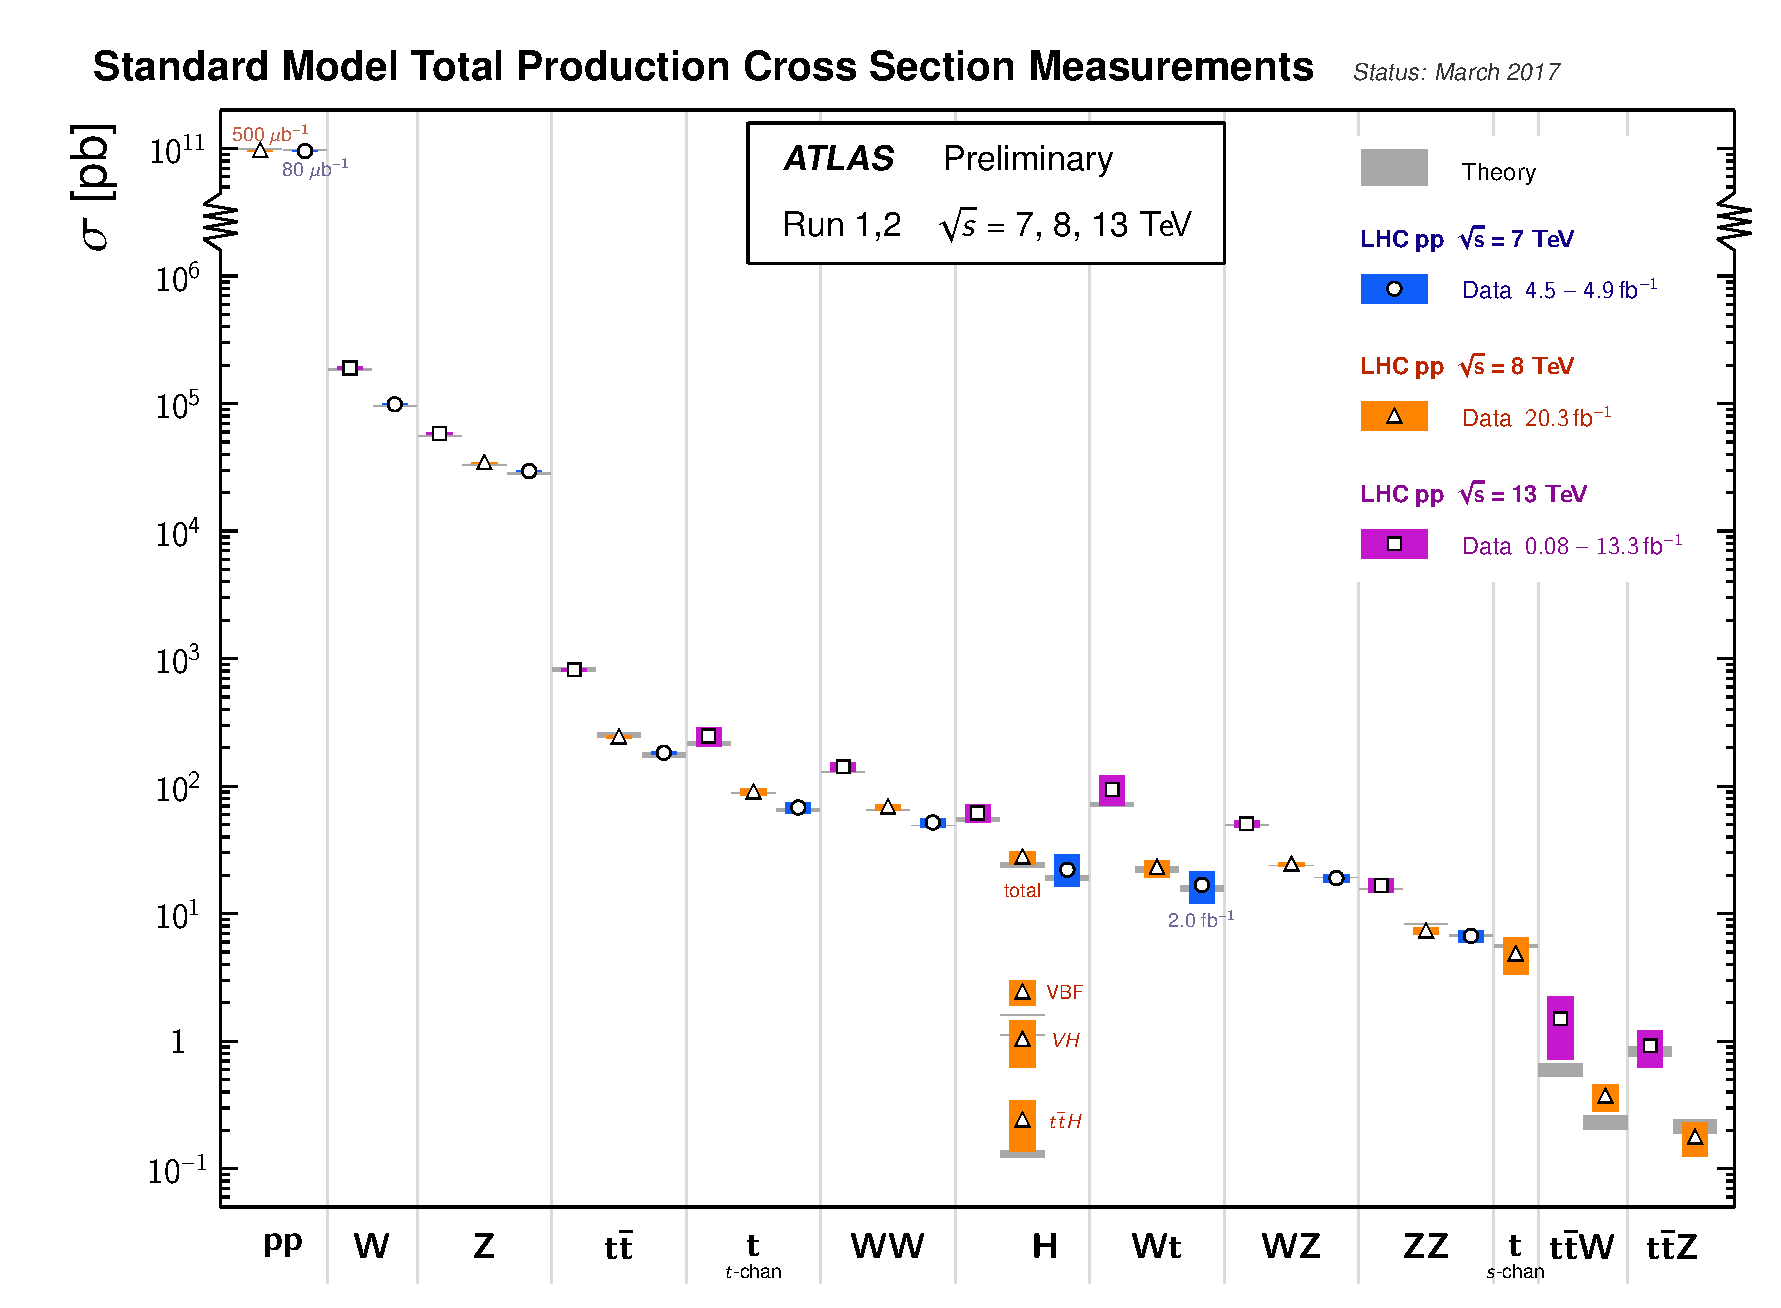
\includegraphics[width=1\textwidth]{images_tmp/cross_section.pdf}
\caption{Resumen de las distintas medidas de sección eficaz de producción de procesos del SM, comparadas con sus valores teóricos esperados \cite{crosssect_web}.}
\label{cross_section}
\end{figure}


\clearpage